\documentclass[t]{beamer}

\usepackage[english]{babel}
\usepackage[utf8]{inputenc}

% ============================================================
% POTASSCO STYLES
% ============================================================
\usepackage{xcolor}

\definecolor{potgreen}{RGB}{157, 163, 34}   % olive green (logo)
\definecolor{potnavy}{RGB}{3,  12,  62}    % dark navy (logo)
\definecolor{potblue}{RGB}{2,   91, 255}    % bright blue (icon)

% Derived / accent
\definecolor{potgreen-light}{RGB}{214, 217, 147}  % tint for backgrounds
\definecolor{potnavy-mid}{HTML}{8F92AC}      % lighter navy for text/borders
\definecolor{potblue-light}{RGB}{200, 215, 255}   % tint for backgrounds


% Clingin colors
\definecolor{clinguinblue}{HTML}{0052CC}
\definecolor{clinguinpurple}{HTML}{6554C0}
\definecolor{clinguingreen}{HTML}{36B37E}
\definecolor{clinguinyellow}{HTML}{FFAB00}
\definecolor{clinguindanger}{HTML}{FF5630}
 %Include to define colors
% ============================================================
% BEAMER THEME — Potassco / University of Potsdam
% ============================================================
% Sections:
%   1. Theme & Logos
%   2. Footer
%   3. Blocks
%   4. Colors
%   5. Formats & Templates
%   6. Section Title Slide
% ============================================================


% ============================================================
% 1. THEME & LOGOS
% ============================================================
\usetheme{default}
\usecolortheme{beaver}

% Logo files — update paths if directory structure changes
\pgfdeclareimage[height=2cm]{potasscologo}{./include/logos/potassco-technologies/Logo/Digital/pt_rgb_2colors_digital.png}
\pgfdeclareimage[height=0.5cm]{potasscoicon}{./include/logos/potassco-technologies/Icon/Digital/pt_icon_rgb_green_digital.png}


% ============================================================
% 2. FOOTER
% ============================================================
% Layout: [author (institute)] [title + page] [logo/page]
% Widths must sum to \paperwidth: .4 + .5 + .1 = 1.0

\setbeamertemplate{headline}{}

\setbeamertemplate{footline}{
  \hbox{\color{white}\rule{\paperwidth}{0.4pt}}%
  \leavevmode%
  \hbox{%
  \begin{beamercolorbox}[wd=.4\paperwidth,ht=2.25ex,dp=1ex,leftskip=6pt]{author in head/foot}%
    \usebeamerfont{author in head/foot}\insertshortauthor\ (\insertshortinstitute)
  \end{beamercolorbox}%
  \begin{beamercolorbox}[wd=.5\paperwidth,ht=2.25ex,dp=1ex,leftskip=6pt]{title in head/foot}%
    \usebeamerfont{title in head/foot}\insertshorttitle\ -- \textit{\insertsectionhead}\hspace{20pt}
  \end{beamercolorbox}%
  \begin{beamercolorbox}[wd=.1\paperwidth,ht=2.25ex,dp=1ex,center]{logo in head/foot}%
    \insertframenumber{} / \inserttotalframenumber\hspace*{1ex}
  \end{beamercolorbox}%
  }%
  \vskip0pt%
}

% Footer colors
\setbeamercolor{author in head/foot}{bg=gray!15, fg=black}
\setbeamercolor{title in head/foot}{bg=gray!10, fg=black}
\setbeamercolor{logo in head/foot}{bg=gray!10, fg=black}


% ============================================================
% 3. BLOCKS
% ============================================================
% Template: [default] = plain rectangles (no shadow/rounding)
% Alternatives: [rounded][shadow=false], [rounded][shadow=true]

\setbeamertemplate{blocks}[default]


\setbeamercolor{block title}{fg=black, bg=potnavy-mid!50}
\setbeamercolor{block body}{fg=black, bg=potnavy-mid!20}
\setbeamercolor{block title example}{fg=black, bg=potgreen-light}
\setbeamercolor{block body example}{fg=black, bg=potgreen!10}
\setbeamercolor{block title alerted}{fg=black, bg=potblue-light}
\setbeamercolor{block body alerted}{fg=black, bg=potblue!8}

\setbeamerfont{block title}{size=\small}
\setbeamerfont{block title example}{size=\small}
\setbeamerfont{block title alerted}{size=\small}
\setbeamerfont{block body}{size=\footnotesize}
\setbeamerfont{block body example}{size=\footnotesize}
\setbeamerfont{block body alerted}{size=\footnotesize}


% ============================================================
% 4. COLORS
% ============================================================

% --- Lists
\setbeamercolor{itemize item}{fg=potnavy}
\setbeamercolor{itemize subitem}{fg=potnavy}
\setbeamercolor{section number projected}{bg=potnavy}
\setbeamercolor{subsection number projected}{bg=potnavy}

% --- Palette (used by some outer themes)
\setbeamercolor{palette primary}{bg=potnavy, fg=white}
\setbeamercolor{palette secondary}{bg=potnavy, fg=white}
\setbeamercolor{palette tertiary}{bg=potnavy!70!white, fg=white}
\setbeamercolor{palette quaternary}{bg=potnavy!60!white, fg=white}

% --- Title & frame title
\setbeamercolor*{title}{bg=white, fg=potnavy}
\setbeamercolor{frametitle}{fg=potnavy, bg=white}

% --- Footnotes
\setbeamercolor{footnote}{fg=black!60}
\setbeamercolor{footnote mark}{fg=black!60}

% --- Text roles
\setbeamercolor{alerted text}{fg=potblue}  % change to potgreen for green alerts
\setbeamercolor{structure}{fg=potnavy}
\setbeamercolor{institute}{fg=potnavy!60}


% ============================================================
% 5. FORMATS & TEMPLATES
% ============================================================

% Remove footnote rule line
\renewcommand\footnoterule{}

% Remove navigation symbols (comment out to restore)
\setbeamertemplate{navigation symbols}{}

% Inner theme: circles for bullet points
% Alternatives: rectangles, inmargin, default
\useinnertheme{circles}

% Table of contents style
\setbeamertemplate{section in toc}{%
  \leavevmode\leftskip=5.65ex%
  \llap{\raisebox{0.2ex}{\textcolor{gray}{$\circ$}}\kern1ex}%
  \inserttocsection\par%
}


% ============================================================
% 6. SECTION TITLE SLIDE
% ============================================================
% Shown automatically before each \section{}
% Remove \AtBeginSection block to disable

\AtBeginSection{
  \begin{frame}
    \vfill
    \bigskip
    \bigskip
    \centering
    \includegraphics[height=2em, keepaspectratio,
      trim=10pt 10pt 10pt 10pt, clip]{./include/logos/potassco-technologies/Icon/Digital/pt_icon_rgb_green_digital.png}%
    \hspace{0.4em}%
    {\usebeamerfont{title}\color{potnavy}\textbf{\LARGE\MakeUppercase{\insertsectionhead}}}
    \vfill
  \end{frame}
}

% Saves the default text color at document start (used in some diagrams)
\AtBeginDocument{\colorlet{defaultcolor}{.}}
 %Include to set beamer theme and color scheme
% %%%%%%%%%%%%%%%%%%%%% Listings
\usepackage{listings}
\input{./include/asp-macros/listings}

\newcommand{\lstbasicstyle}{\ttfamily\scriptsize}

\usepackage{caption}

\captionsetup[lstlisting]{position=top,justification=raggedleft,singlelinecheck=false,labelformat=empty,font={scriptsize,tt},skip=0pt}


\lstdefinelanguage{clingos}{%
  language=clingo,
  basicstyle=\lstbasicstyle,
  aboveskip=1.5em,
  belowskip=1em,
  commentstyle={\color{potnavy-mid}\itshape}
}

\lstset{
  columns=fullflexible,
  numberblanklines=false,
  xleftmargin=0.1cm,
  framesep=4pt,
  frame=single,
  numbers=none,
  basicstyle=\lstbasicstyle,
  escapeinside={(*@}{@*)}
}



% ============================================================
% PRIMITIVE styles — named by color, no semantics
% Use these when you need direct color control per-slide
% ============================================================

\lstdefinestyle{blue-dark}{
  backgroundcolor=\color{potnavy},
  language=clingos,
  basicstyle=\lstbasicstyle\color{white},
  rulecolor=\color{potnavy},
  escapeinside={(*@}{@*)},
}
\lstdefinestyle{blue-mid}{
  backgroundcolor=\color{potnavy-mid!30},
  language=clingos,
  basicstyle=\lstbasicstyle\color{potnavy},
  rulecolor=\color{potnavy},
  escapeinside={(*@}{@*)},
}
\lstdefinestyle{blue-light}{
  backgroundcolor=\color{potblue-light},
  language=clingos,
  basicstyle=\lstbasicstyle\color{potnavy},
  rulecolor=\color{potnavy},
  escapeinside={(*@}{@*)},
}
\lstdefinestyle{blue-outline}{
  language=clingos,
  basicstyle=\lstbasicstyle\color{potblue},
  frame=single,
  rulecolor=\color{potblue},
  escapeinside={(*@}{@*)},
}
\lstdefinestyle{green-dark}{
  backgroundcolor=\color{potgreen},
  language=clingos,
  basicstyle=\lstbasicstyle\color{white},
  rulecolor=\color{potgreen},
  escapeinside={(*@}{@*)},
}
\lstdefinestyle{green-light}{
  backgroundcolor=\color{potgreen-light},
  language=clingos,
  basicstyle=\lstbasicstyle\color{potnavy},
  rulecolor=\color{potgreen},
  escapeinside={(*@}{@*)},
}
\lstdefinestyle{green-outline}{
  language=clingos,
  basicstyle=\lstbasicstyle\color{potgreen},
  frame=single,
  rulecolor=\color{potgreen},
  escapeinside={(*@}{@*)},
}

% shell
\lstdefinestyle{console}{
  frame=none,
  language=sh,
  basicstyle=\lstbasicstyle\color{potnavy-mid},
  linewidth=14cm,
  escapeinside={(*@}{@*)}
}

% ============================================================
% SEMANTIC styles — named by role, defined in terms of above
% Use these as defaults; override per-slide with primitives
% ============================================================

 %Include if you want to use listings
\usepackage{tikz}
% ============================================================
% TIKZ STYLES
% ============================================================
\tikzset{
  % --- PRIMITIVES (color-named) ---
  blue-dark/.style={
    fill=potnavy,
    draw=potnavy,
    text=white,
    font=\scriptsize,
    inner sep=5pt,
    align=center
  },
  blue-mid/.style={
    fill=potnavy-mid!30,
    draw=potnavy-mid,
    text=potnavy,
    font=\scriptsize,
    inner sep=5pt,
    align=center
  },
  blue-light/.style={
    fill=potblue-light,
    draw=potnavy-mid,
    text=potnavy,
    font=\scriptsize,
    inner sep=5pt,
    align=center
  },
  blue-outline/.style={
    fill=white,
    draw=potblue,
    text=potblue,
    font=\scriptsize,
    inner sep=5pt,
    align=center
  },
  green-dark/.style={
    fill=potgreen,
    draw=potgreen,
    text=white,
    font=\scriptsize,
    inner sep=5pt,
    align=center
  },
  green-light/.style={
    fill=potgreen-light,
    draw=potgreen,
    text=potnavy,
    font=\scriptsize,
    inner sep=5pt,
    align=center
  },
  green-outline/.style={
    fill=white,
    draw=potgreen,
    text=potgreen,
    font=\scriptsize,
    inner sep=5pt,
    align=center
  },
  % --- SECTION LABELS ---
  % section container box
  section-box/.style={
    draw=potnavy,
    rounded corners,
    fill=potnavy,
    fill opacity=0.04
  },
  % section box label node
  section-label/.style={
    blue-dark,
    rounded corners,
    font=\tiny\bfseries,
    inner sep=3pt,
    anchor=north west
  },
  section/.style={blue-dark},
  subsection/.style={blue-mid},
  section-title/.style={
    font=\scriptsize\bfseries,
    text=potnavy
  },
  subsection-title/.style={
    font=\scriptsize,
    text=potnavy-mid,
    align=center
  },
  section-info/.style={
    font=\tiny,
    text=potnavy-mid,
    align=left
  },
  % --- ARROWS ---
  arrw/.style={
    draw=potblue,
    font=\tiny,
    -latex
  },
  subarrw/.style={
    draw=potnavy-mid,
    opacity=0.6,
    densely dotted,
    -latex
  },
  arrw-system/.style={
    draw=potnavy,
    dotted,
    -latex
  },
  % --- GRID ---
  grid/.style={
    gray,
    very thin,
    opacity=0.1
  },
  % --- SEMANTIC (role-named) ---
  encoding/.style={blue-light},
  encoding2/.style={blue-mid},
  input/.style={green-outline},
  output/.style={green-dark},
  system/.style={
    blue-dark,
    double,
    rounded corners
  },
  action/.style={
    fill=potblue,
    draw=potblue,
    text=white,
    double,
    rounded corners,
    font=\tiny,
    inner sep=3pt,
    align=center
  },
}
 %Include if you want to use TikZ !!!After macros

% \input{macro}

% ============================================================
% TITLE
% ============================================================
\title[Short Title]{Full Title}
\author[Short Names]{Full Names}
\institute[KRR@UP]{University of Potsdam \&\ Potassco Solutions GmbH \\
  \bigskip
  \pgfuseimage{potasscologo}}
\date{}

% ============================================================
% DOCUMENT
% ============================================================
\begin{document}
% ----------------------------------------------------------------------
\frame{\titlepage}
% ----------------------------------------------------------------------
\begin{frame}{Outline}
  \bigskip
  \vfill
  \tableofcontents
\end{frame}

% ----------------------------------------------------------------------
\section{Introduction}
% ----------------------------------------------------------------------
\begin{frame}{Motivation}
\end{frame}
% ----------------------------------------------------------------------
\section{Preliminaries}
% ----------------------------------------------------------------------
\begin{frame}{}
\end{frame}
% ----------------------------------------------------------------------
\section{Summary}
% ---------------------------------------------------------------------
\begin{frame}{Summary}
  \begin{itemize}
  \item \url{potassco.org}
  \end{itemize}
\end{frame}

% ----------------------------------------------------------------------
\section{Style examples}
% ----------------------------------------------------------------------

% ============================================================
\begin{frame}{Blocks}

  \begin{block}{Regular Block}
    This is a regular block with \alert{alerted text} and normal content.
  \end{block}

  \begin{exampleblock}{Example Block}
    This is an example block, good for encodings or definitions.
  \end{exampleblock}

  \begin{alertblock}{Alert Block}
    This is an alert block, good for warnings or key results.
  \end{alertblock}

\end{frame}

% ============================================================
\begin{frame}{Itemize \& Enumerate}

  \begin{columns}
    \column{0.5\textwidth}
      Itemize:
      \begin{itemize}
        \item First item
        \item Second item with \alert{alert}
          \begin{itemize}
            \item Nested item
            \item Another nested
          \end{itemize}
        \item Third item
      \end{itemize}

    \column{0.5\textwidth}
      Enumerate:
      \begin{enumerate}
        \item First step
        \item Second step
          \begin{enumerate}
            \item Sub-step a
            \item Sub-step b
          \end{enumerate}
        \item Third step
      \end{enumerate}
  \end{columns}

\end{frame}

% ============================================================
\begin{frame}{Columns}

  \begin{columns}[T]
    \column{0.33\textwidth}
      \begin{block}{Column 1}
        Left column content. Can hold text, lists, or code.
      \end{block}
      \begin{itemize}
        \item item one
        \item item two
      \end{itemize}

    \column{0.33\textwidth}
      \begin{exampleblock}{Column 2}
        Middle column content.
      \end{exampleblock}
      Some regular text below the block.

    \column{0.33\textwidth}
      \begin{alertblock}{Column 3}
        Right column content.
      \end{alertblock}
      \begin{enumerate}
        \item step one
        \item step two
      \end{enumerate}
  \end{columns}

\end{frame}


% ============================================================
\begin{frame}{Theorem, Definition \& Proof}

  \begin{definition}
    A \alert{stable model} of a program $P$ is a minimal model of
    the reduct $P^M$ for some interpretation $M$.
  \end{definition}

  \begin{theorem}
    For any program $P$, if $M$ is a stable model of $P$ then
    $M \models P$.
  \end{theorem}

  \begin{proof}
    By construction of the GL reduct $P^M$, every rule head
    supported by $M$ is derivable from $P^M$. Minimality
    follows from the definition of stable models. \qed
  \end{proof}

\end{frame}


\begin{frame}[fragile]{Listings Style Reference}

\tiny
\textit{default}
\begin{lstlisting}[language=clingos]
a(1). b(X) :- a(X). #show b/1.
% Comment
\end{lstlisting}


\textit{blue-dark}
\begin{lstlisting}[style=blue-dark]
a(1). b(X) :- a(X). #show b/1.
\end{lstlisting}
\textit{blue-mid}
\begin{lstlisting}[style=blue-mid]
a(1). b(X) :- a(X). #show b/1.
\end{lstlisting}
\textit{blue-light}
\begin{lstlisting}[style=blue-light]
a(1). b(X) :- a(X). #show b/1.
\end{lstlisting}
\textit{blue-outline}
\begin{lstlisting}[style=blue-outline]
a(1). b(X) :- a(X). #show b/1.
\end{lstlisting}

\end{frame}
\begin{frame}[fragile]{Listings Style Reference (cont.)}
\textit{green-dark}
\begin{lstlisting}[style=green-dark]
a(1). b(X) :- a(X). #show b/1.
\end{lstlisting}
\textit{green-light}
\begin{lstlisting}[style=green-light]
a(1). b(X) :- a(X). #show b/1.
\end{lstlisting}
\textit{green-outline}
\begin{lstlisting}[style=green-outline]
a(1). b(X) :- a(X). #show b/1.
\end{lstlisting}
\textit{console}
\begin{lstlisting}[style=console]
$ clingo example.lp
clingo version 5.5.0
Reading from example.lp
Solving...
Answer: 1
b(1)
SATISFIABLE
\end{lstlisting}


\end{frame}

\begin{frame}{Style Reference — TikZ Base Nodes}
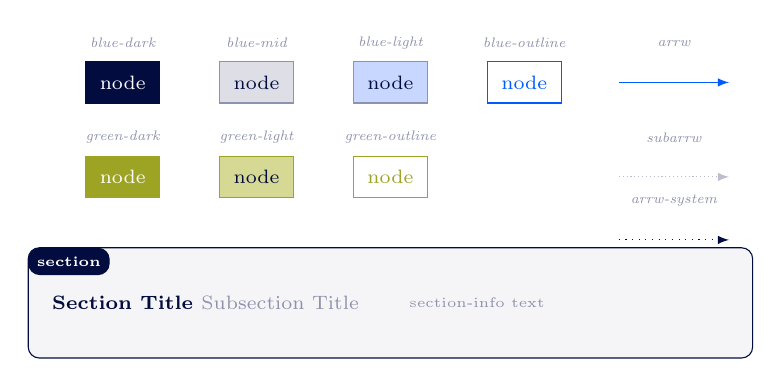
\begin{tikzpicture}[node distance=1.5cm]

  % --- blue row
  \node[font=\tiny\itshape, text=potnavy-mid] at (1.5, 4.3) {blue-dark};
  \node[blue-dark]    at (1.5, 3.8) {node};
  \node[font=\tiny\itshape, text=potnavy-mid] at (3.2, 4.3) {blue-mid};
  \node[blue-mid]     at (3.2, 3.8) {node};
  \node[font=\tiny\itshape, text=potnavy-mid] at (4.9, 4.3) {blue-light};
  \node[blue-light]   at (4.9, 3.8) {node};
  \node[font=\tiny\itshape, text=potnavy-mid] at (6.6, 4.3) {blue-outline};
  \node[blue-outline] at (6.6, 3.8) {node};
  % --- green row
  \node[font=\tiny\itshape, text=potnavy-mid] at (1.5, 3.1) {green-dark};
  \node[green-dark]    at (1.5, 2.6) {node};
  \node[font=\tiny\itshape, text=potnavy-mid] at (3.2, 3.1) {green-light};
  \node[green-light]   at (3.2, 2.6) {node};
  \node[font=\tiny\itshape, text=potnavy-mid] at (4.9, 3.1) {green-outline};
  \node[green-outline] at (4.9, 2.6) {node};
  % --- section label styles + grouping example
  \draw[section-box] (0.3, 0.3) rectangle (9.5, 1.7);
  \node[section-label] at (0.3, 1.7) {section};
  \node[section-title]    at (1.5, 1) {Section Title};
  \node[subsection-title] at (3.5, 1) {Subsection Title};
  \node[section-info]     at (6.0, 1) {section-info text};
  % --- arrows
  \node[font=\tiny\itshape, text=potnavy-mid] at (8.5, 4.3) {arrw};
  \draw[arrw] (7.8, 3.8) -- (9.2, 3.8);
  \node[font=\tiny\itshape, text=potnavy-mid] at (8.5, 3.1) {subarrw};
  \draw[subarrw] (7.8, 2.6) -- (9.2, 2.6);
  \node[font=\tiny\itshape, text=potnavy-mid] at (8.5, 2.3) {arrw-system};
  \draw[arrw-system] (7.8, 1.8) -- (9.2, 1.8);

\end{tikzpicture}
\end{frame}
\begin{frame}{Style Reference — Tikz custom nodes}
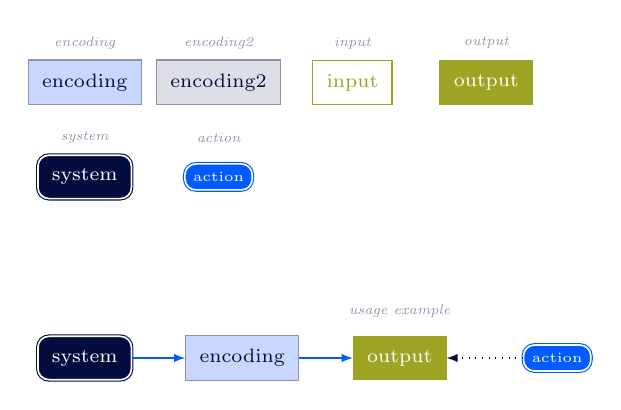
\begin{tikzpicture}[node distance=1.5cm]
  % --- semantic nodes row 1
  \node[font=\tiny\itshape, text=potnavy-mid] at (1.5, 4.3) {encoding};
  \node[encoding]  at (1.5, 3.8) {encoding};
  \node[font=\tiny\itshape, text=potnavy-mid] at (3.2, 4.3) {encoding2};
  \node[encoding2] at (3.2, 3.8) {encoding2};
  \node[font=\tiny\itshape, text=potnavy-mid] at (4.9, 4.3) {input};
  \node[input]     at (4.9, 3.8) {input};
  \node[font=\tiny\itshape, text=potnavy-mid] at (6.6, 4.3) {output};
  \node[output]    at (6.6, 3.8) {output};
  % --- semantic nodes row 2
  \node[font=\tiny\itshape, text=potnavy-mid] at (1.5, 3.1) {system};
  \node[system]    at (1.5, 2.6) {system};
  \node[font=\tiny\itshape, text=potnavy-mid] at (3.2, 3.1) {action};
  \node[action]    at (3.2, 2.6) {action};
  % --- usage example with arrows
  \node[font=\tiny\itshape, text=potnavy-mid] at (5.5, 0.9) {usage example};
  \node[system]   (sys)  at (1.5, 0.3) {system};
  \node[encoding] (enc)  at (3.5, 0.3) {encoding};
  \node[output]   (out)  at (5.5, 0.3) {output};
  \node[action]   (act)  at (7.5, 0.3) {action};
  \draw[arrw]      (sys) -- (enc);
  \draw[arrw]      (enc) -- (out);
  \draw[arrw-system] (act) -- (out);
\end{tikzpicture}
\end{frame}


\end{document}

%%% Local Variables:
%%% mode: latex
%%% TeX-master: t
%%% TeX-PDF-mode: t
%%% End:
